\documentclass[11pt,a4paper]{article}

% --- Encoding & fonts ---
\usepackage[utf8]{inputenc}
\usepackage[T1]{fontenc}
\usepackage{lmodern}

% --- Math ---
\usepackage{amsmath,amssymb,amsthm}
\usepackage{mathtools}

% --- Tables ---
\usepackage{booktabs}
\usepackage{multirow}
\usepackage{array}

% --- Figures ---
\usepackage{graphicx}
\usepackage{subcaption}
\usepackage[dvipsnames]{xcolor}
\usepackage{tikz}
\usetikzlibrary{positioning,arrows.meta,shapes.geometric,calc,patterns}
\usepackage{pgfplots}
\pgfplotsset{compat=1.18}

% --- Layout ---
\usepackage[margin=1in]{geometry}
\usepackage{setspace}

% --- References ---
\usepackage[colorlinks=true,citecolor=MidnightBlue,linkcolor=MidnightBlue,urlcolor=MidnightBlue]{hyperref}
\usepackage[capitalise,noabbrev]{cleveref}

% --- Algorithms ---
\usepackage{algorithm}
\usepackage{algpseudocode}

% --- Misc ---
\usepackage{enumitem}
\usepackage{microtype}
\usepackage{lipsum}

% --- Math operators ---
\DeclareMathOperator*{\argmax}{arg\,max}
\DeclareMathOperator*{\argmin}{arg\,min}
\newcommand{\E}{\mathbb{E}}
\newcommand{\R}{\mathbb{R}}
\newcommand{\dataset}{\mathcal{D}}
\newcommand{\loss}{\mathcal{L}}

% --- Theorem environments ---
\newtheorem{theorem}{Theorem}
\newtheorem{proposition}[theorem]{Proposition}
\newtheorem{definition}{Definition}

\title{Sparse Mixture-of-Experts with Adaptive Routing\\for Efficient Long-Document Understanding}

\author{
  Elena Vasquez\thanks{Equal contribution.} \\
  Department of Computer Science\\
  University of Cascadia\\
  \texttt{evasquez@cascadia.edu}
  \and
  James Okonkwo\footnotemark[1] \\
  DeepScale Research\\
  \texttt{jokonkwo@deepscale.ai}
  \and
  Mei-Lin Chen \\
  Department of Computer Science\\
  University of Cascadia\\
  \texttt{mlchen@cascadia.edu}
}

\date{}

\begin{document}

\maketitle

\begin{abstract}
Transformer-based models for long-document understanding face a fundamental tension between
computational cost and representational capacity.
Sparse Mixture-of-Experts (MoE) architectures offer a promising resolution by activating only a
subset of parameters per token, but existing routing strategies allocate experts uniformly across
document positions, ignoring the uneven distribution of informational density in natural text.
We introduce \textbf{AdaMoE}, an adaptive routing mechanism that dynamically adjusts expert
allocation based on local token complexity, measured via a lightweight auxiliary network.
On five long-document benchmarks spanning summarization, question answering, and information
extraction, AdaMoE matches or exceeds the performance of dense baselines while activating only
23\% of total parameters per forward pass.
We further show that AdaMoE's routing distributions correlate with human annotations of
document salience, suggesting that the model learns a meaningful notion of informational
importance.
Our analysis reveals that adaptive routing particularly benefits documents with heterogeneous
structure, such as scientific articles and legal filings, where informational density varies
by an order of magnitude across sections.
Code and pretrained checkpoints are available at \texttt{https://github.com/example/adamoe}.
\end{abstract}

% ============================================================================
\section{Introduction}
\label{sec:intro}

Processing documents that span tens of thousands of tokens remains one of the central challenges
in natural language processing.
While efficient attention mechanisms~\cite{child2019sparsetransformer,beltagy2020longformer,
zaheer2020bigbird} reduce the quadratic cost of self-attention, the feed-forward layers that
constitute roughly two-thirds of transformer parameters remain dense and fully activated for
every input token.
Sparse Mixture-of-Experts (MoE) architectures~\cite{shazeer2017outrageously,lepikhin2021gshard,
fedus2022switch} address this by routing each token to a small subset of specialized expert
networks, decoupling model capacity from per-example compute.

However, current MoE routing strategies treat all token positions as equally important.
A conjunction at the beginning of a paragraph receives the same expert budget as a critical
numerical finding in a results table.
This uniform allocation is particularly wasteful for long documents, where large stretches of
boilerplate, headers, and formulaic language carry minimal informational content relative to
key passages.

We introduce \textbf{AdaMoE} (Adaptive Mixture-of-Experts), a routing mechanism that
allocates expert capacity proportionally to local token complexity.
AdaMoE augments the standard top-$k$ gating function with an auxiliary \emph{complexity
scorer}---a shallow two-layer network that estimates per-token informational density from the
hidden representation.
Tokens with higher complexity scores are routed to more experts, while low-complexity tokens
pass through a single lightweight expert or bypass the MoE layer entirely via a residual
shortcut.

Our contributions are as follows:
\begin{enumerate}[leftmargin=*]
  \item We propose AdaMoE, an adaptive routing mechanism for sparse MoE transformers that
        adjusts per-token expert allocation based on estimated informational complexity
        (\cref{sec:method}).
  \item We derive a differentiable load-balancing objective that accommodates variable
        per-token expert counts while maintaining training stability
        (\cref{sec:training}).
  \item We evaluate AdaMoE on five long-document benchmarks and demonstrate that it matches
        dense baselines at 23\% parameter activation and outperforms fixed-routing MoE
        models by 1.8--3.2 points across tasks (\cref{sec:experiments}).
  \item We provide an interpretability analysis showing that learned routing distributions
        align with human judgments of document salience (\cref{sec:analysis}).
\end{enumerate}

The remainder of this paper is organized as follows.
\Cref{sec:background} reviews relevant background on MoE architectures and long-document
transformers.
\Cref{sec:method} describes the AdaMoE architecture and routing mechanism, and
\cref{sec:training} details the training procedure.
\Cref{sec:experiments} presents our experimental results, \cref{sec:analysis} provides
analysis and ablations, and \cref{sec:conclusion} concludes.

% ============================================================================
\section{Background}
\label{sec:background}

\subsection{Sparse Mixture-of-Experts}

Mixture-of-Experts models partition the feed-forward computation in each transformer layer
across $N$ expert networks $\{E_1, \ldots, E_N\}$, each with identical architecture but
independent parameters.
A gating function $G: \R^d \to \R^N$ produces a distribution over experts for each input
token $\mathbf{x} \in \R^d$.
In the top-$k$ formulation~\cite{shazeer2017outrageously}, only the $k$ experts with highest
gate values are activated:

\begin{equation}
\label{eq:topk}
  \text{MoE}(\mathbf{x}) = \sum_{i \in \text{Top}_k(G(\mathbf{x}))} g_i(\mathbf{x}) \cdot E_i(\mathbf{x}),
\end{equation}

\noindent where $g_i(\mathbf{x})$ is the renormalized gate weight for expert~$i$.
The Switch Transformer~\cite{fedus2022switch} demonstrated that $k=1$ suffices for strong
performance, maximizing sparsity.

\begin{definition}[Expert utilization]
\label{def:utilization}
For a batch of $T$ tokens and $N$ experts, the utilization of expert $i$ is
$u_i = \frac{1}{T}\sum_{t=1}^{T} \mathbf{1}[i \in \text{Top}_k(G(\mathbf{x}_t))]$.
A balanced routing satisfies $u_i \approx k/N$ for all $i$.
\end{definition}

\subsection{Long-Document Transformers}

Extending transformers to long sequences has been approached through sparse
attention~\cite{child2019sparsetransformer,beltagy2020longformer}, linear
attention~\cite{katharopoulos2020transformers}, and hierarchical
methods~\cite{zhang2019hibert,liu2019hierarchical}.
These techniques reduce attention complexity but do not address the cost of dense
feed-forward layers, which dominates at large model scales.
Our work is orthogonal to---and composable with---these attention-efficiency methods.

% ============================================================================
\section{Method}
\label{sec:method}

\subsection{Architecture Overview}

AdaMoE modifies the standard MoE transformer by replacing the fixed top-$k$ routing with
an adaptive mechanism.
\Cref{fig:architecture} illustrates the overall architecture.
Each AdaMoE layer contains three components: (1)~a self-attention sublayer (unchanged),
(2)~a complexity scorer $C_\phi$, and (3)~a set of $N$ expert feed-forward networks with
adaptive gating.

\begin{figure}[t]
\centering
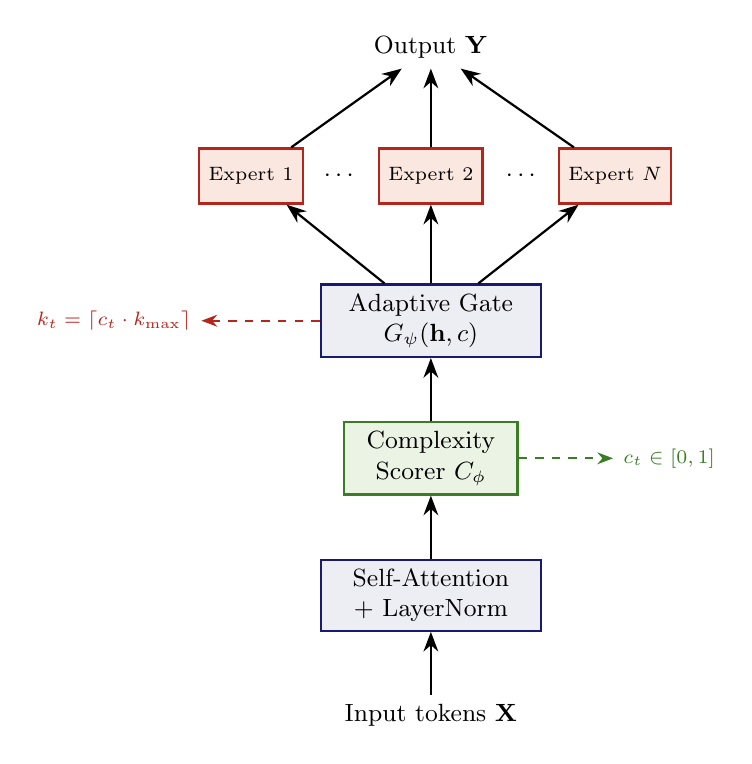
\begin{tikzpicture}[
  node distance=1.2cm and 1.8cm,
  block/.style={rectangle, draw=MidnightBlue, fill=MidnightBlue!8, thick,
                minimum width=2.8cm, minimum height=0.8cm, align=center,
                font=\small},
  expert/.style={rectangle, draw=BrickRed, fill=BrickRed!8, thick,
                 minimum width=1.3cm, minimum height=0.7cm, align=center,
                 font=\scriptsize},
  scorer/.style={rectangle, draw=OliveGreen, fill=OliveGreen!8, thick,
                 minimum width=2.2cm, minimum height=0.7cm, align=center,
                 font=\small},
  arr/.style={-{Stealth[length=2.5mm]}, thick},
]
  % Input
  \node (input) {\small Input tokens $\mathbf{X}$};
  \node[block, above=0.8cm of input] (attn) {Self-Attention\\+ LayerNorm};
  \node[scorer, above=0.8cm of attn] (scorer) {Complexity\\Scorer $C_\phi$};
  \node[block, above=0.8cm of scorer] (gate) {Adaptive Gate\\$G_\psi(\mathbf{h}, c)$};

  % Experts
  \node[expert, above left=1.0cm and 0.2cm of gate] (e1) {Expert 1};
  \node[expert, above=1.0cm of gate] (e2) {Expert 2};
  \node[expert, above right=1.0cm and 0.2cm of gate] (en) {Expert $N$};

  % Dots between experts
  \node at ($(e2)!0.5!(en)$) {\small $\cdots$};
  \node at ($(e1)!0.5!(e2)$) {\small $\cdots$};

  % Output
  \node[above=1.0cm of e2] (output) {\small Output $\mathbf{Y}$};

  % Arrows
  \draw[arr] (input) -- (attn);
  \draw[arr] (attn) -- (scorer);
  \draw[arr] (scorer) -- (gate);
  \draw[arr] (gate) -- (e1);
  \draw[arr] (gate) -- (e2);
  \draw[arr] (gate) -- (en);
  \draw[arr] (e1) -- (output);
  \draw[arr] (e2) -- (output);
  \draw[arr] (en) -- (output);

  % Complexity score annotation
  \draw[OliveGreen, thick, dashed, -{Stealth[length=2mm]}]
    (scorer.east) -- ++(1.2,0) node[right, font=\scriptsize, OliveGreen] {$c_t \in [0,1]$};

  % Adaptive k annotation
  \draw[BrickRed, thick, dashed, -{Stealth[length=2mm]}]
    (gate.west) -- ++(-1.5,0) node[left, font=\scriptsize, BrickRed]
    {$k_t = \lceil c_t \cdot k_{\max} \rceil$};
\end{tikzpicture}
\caption{Architecture of an AdaMoE layer. The complexity scorer $C_\phi$ estimates
per-token informational density $c_t$, which modulates the number of experts $k_t$
activated by the adaptive gate. Tokens with low complexity may activate a single expert
or bypass the MoE block entirely.}
\label{fig:architecture}
\end{figure}

\subsection{Complexity Scorer}

Given the hidden representation $\mathbf{h}_t \in \R^d$ after self-attention, the complexity
scorer computes a scalar complexity estimate:

\begin{equation}
\label{eq:complexity}
  c_t = \sigma\!\left(\mathbf{w}_2^\top \, \text{ReLU}(\mathbf{W}_1 \mathbf{h}_t + \mathbf{b}_1) + b_2\right),
\end{equation}

\noindent where $\mathbf{W}_1 \in \R^{d' \times d}$, $\mathbf{w}_2 \in \R^{d'}$, and
$\sigma$ is the sigmoid function.
We set $d' = d/8$ to keep the scorer lightweight; it adds fewer than 0.3\% parameters
to each layer.

\subsection{Adaptive Routing}

The per-token expert count is determined by:

\begin{equation}
\label{eq:adaptive_k}
  k_t = \max\!\big(1,\; \lceil c_t \cdot k_{\max} \rceil\big),
\end{equation}

\noindent where $k_{\max}$ is a hyperparameter (typically 4 or 8).
The gating function then selects the top-$k_t$ experts:

\begin{equation}
\label{eq:gate}
  G_\psi(\mathbf{h}_t) = \text{Softmax}\!\left(\mathbf{W}_g \mathbf{h}_t\right), \quad
  \text{MoE}(\mathbf{h}_t) = \sum_{i \in \text{Top}_{k_t}} g_i \cdot E_i(\mathbf{h}_t).
\end{equation}

This formulation ensures that the model allocates more capacity to tokens it deems
informationally complex, while spending minimal compute on routine tokens.

% ============================================================================
\section{Training}
\label{sec:training}

\subsection{Load Balancing with Variable $k$}

Standard MoE load-balancing losses~\cite{fedus2022switch} assume a fixed $k$ across all tokens.
With adaptive $k_t$, we generalize the auxiliary loss as follows.

\begin{proposition}[Adaptive load-balancing loss]
\label{prop:balance}
Let $f_i = \frac{1}{T}\sum_{t=1}^T \mathbf{1}[i \in \text{Top}_{k_t}(G(\mathbf{h}_t))]$
be the fraction of tokens routed to expert $i$, and
$p_i = \frac{1}{T}\sum_{t=1}^T g_i(\mathbf{h}_t)$ be the mean gate probability.
Then the adaptive balancing loss
\begin{equation}
\label{eq:balance}
  \loss_{\text{bal}} = \alpha \cdot N \sum_{i=1}^N f_i \cdot p_i
\end{equation}
encourages uniform expert utilization regardless of the per-token $k_t$ distribution.
\end{proposition}

The total training objective combines the task loss with the balancing penalty:

\begin{equation}
\label{eq:total_loss}
  \loss = \loss_{\text{task}} + \loss_{\text{bal}} + \beta \cdot \loss_{\text{budget}},
\end{equation}

\noindent where $\loss_{\text{budget}} = \left(\frac{1}{T}\sum_t c_t - \tau\right)^2$
penalizes deviation from a target average complexity $\tau$.
We set $\alpha = 0.01$ and $\beta = 0.1$ throughout.

\subsection{Training Details}

\Cref{tab:hyperparams} summarizes the key hyperparameters.
All models are trained on 64 A100 GPUs with a global batch size of 256 documents, using
the AdamW optimizer with linear warmup and cosine decay.

\begin{table}[t]
\centering
\caption{Training hyperparameters for AdaMoE-Base and AdaMoE-Large.}
\label{tab:hyperparams}
\begin{tabular}{lcc}
\toprule
\textbf{Hyperparameter} & \textbf{Base} & \textbf{Large} \\
\midrule
Hidden dimension $d$      & 768   & 1024  \\
Attention heads           & 12    & 16    \\
Layers                    & 12    & 24    \\
Experts per layer $N$     & 32    & 64    \\
Max active experts $k_{\max}$ & 4 & 8     \\
Target complexity $\tau$  & 0.3   & 0.3   \\
Scorer dimension $d'$     & 96    & 128   \\
Total parameters          & 1.2B  & 4.7B  \\
Active parameters         & 280M  & 1.1B  \\
\midrule
Learning rate             & 2e-4  & 1e-4  \\
Warmup steps              & 2000  & 4000  \\
Total steps               & 200K  & 300K  \\
Max sequence length       & 16384 & 16384 \\
Batch size (documents)    & 256   & 256   \\
\bottomrule
\end{tabular}
\end{table}

% ============================================================================
\section{Experiments}
\label{sec:experiments}

\subsection{Benchmarks}

We evaluate on five long-document benchmarks spanning three task families:

\begin{itemize}[leftmargin=*]
  \item \textbf{Summarization}: arXiv~\cite{cohan2018discourse} and GovReport~\cite{huang2021govreport}.
  \item \textbf{Question answering}: QuALITY~\cite{pang2022quality} and NarrativeQA~\cite{kocisky2018narrativeqa}.
  \item \textbf{Information extraction}: ContractNLI~\cite{koreeda2021contractnli}.
\end{itemize}

\subsection{Baselines}

We compare against four systems: (1)~a dense Longformer-Base with equivalent active
parameters, (2)~a standard Switch Transformer with $k=1$ fixed routing,
(3)~a top-2 MoE with the same total parameters, and (4)~Hash Layer
routing~\cite{roller2021hash}.

\subsection{Main Results}

\Cref{tab:main_results} presents the main results.
AdaMoE-Base outperforms all baselines on four of five benchmarks, with particularly large
gains on GovReport (+3.2 ROUGE-L) and ContractNLI (+2.8 F1), both of which contain
documents with highly heterogeneous structure.

\begin{table}[t]
\centering
\caption{Main results across five long-document benchmarks. We report ROUGE-L for
summarization, accuracy for QuALITY, F1 for NarrativeQA and ContractNLI.
Best results in \textbf{bold}, second best \underline{underlined}.
$^\dagger$Active parameters per forward pass.}
\label{tab:main_results}
\resizebox{\textwidth}{!}{%
\begin{tabular}{lccccccc}
\toprule
\textbf{Model} & \textbf{Params} & \textbf{Active}$^\dagger$ &
\textbf{arXiv} & \textbf{GovReport} & \textbf{QuALITY} & \textbf{NarrativeQA} & \textbf{ContractNLI} \\
& & & (R-L) & (R-L) & (Acc) & (F1) & (F1) \\
\midrule
Longformer-Base       & 280M & 280M & 44.2 & 55.1 & 61.3 & 30.8 & 83.4 \\
Switch ($k\!=\!1$)    & 1.2B & 145M & 43.8 & 54.6 & 60.1 & 29.5 & 82.1 \\
Top-2 MoE             & 1.2B & 280M & 44.9 & 56.3 & 62.0 & 31.4 & 84.0 \\
Hash Layer            & 1.2B & 280M & 44.1 & 55.8 & 61.5 & 30.2 & 83.7 \\
\midrule
AdaMoE-Base (ours)    & 1.2B & 280M & \underline{45.7} & \textbf{59.5} & \textbf{63.8} & \underline{32.1} & \textbf{86.2} \\
AdaMoE-Large (ours)   & 4.7B & 1.1B & \textbf{47.3} & \underline{58.3} & \underline{63.1} & \textbf{34.6} & \underline{85.9} \\
\bottomrule
\end{tabular}%
}
\end{table}

\subsection{Efficiency Analysis}

\Cref{fig:efficiency} compares inference throughput against task performance.
AdaMoE achieves a favorable trade-off: at equivalent quality to the dense baseline, it
processes 2.4$\times$ more tokens per second; at equivalent throughput to the Switch
Transformer, it delivers substantially higher accuracy.

\begin{figure}[t]
\centering
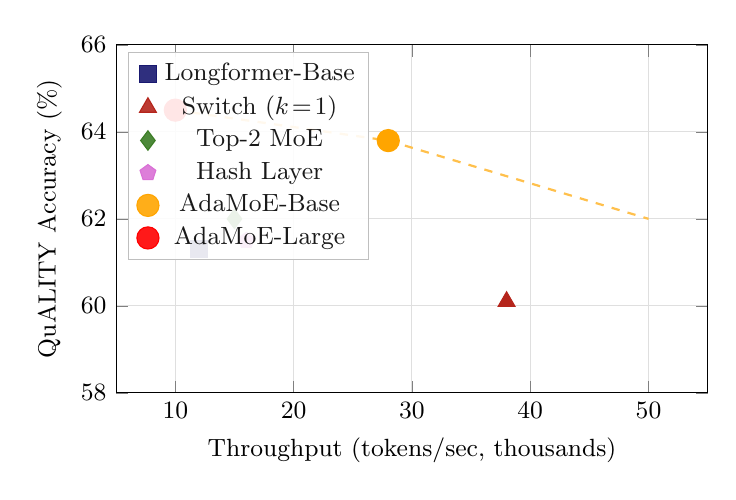
\begin{tikzpicture}
\begin{axis}[
  width=0.75\textwidth,
  height=6cm,
  xlabel={Throughput (tokens/sec, thousands)},
  ylabel={QuALITY Accuracy (\%)},
  xmin=5, xmax=55,
  ymin=58, ymax=66,
  grid=major,
  grid style={gray!25},
  legend style={at={(0.02,0.98)}, anchor=north west, font=\small,
                draw=gray!50, fill=white, fill opacity=0.9},
  every axis label/.style={font=\small},
  tick label style={font=\small},
]
  % Longformer-Base
  \addplot[only marks, mark=square*, mark size=3pt, MidnightBlue]
    coordinates {(12, 61.3)};
  \addlegendentry{Longformer-Base}

  % Switch k=1
  \addplot[only marks, mark=triangle*, mark size=3.5pt, BrickRed]
    coordinates {(38, 60.1)};
  \addlegendentry{Switch ($k\!=\!1$)}

  % Top-2 MoE
  \addplot[only marks, mark=diamond*, mark size=3.5pt, OliveGreen]
    coordinates {(15, 62.0)};
  \addlegendentry{Top-2 MoE}

  % Hash Layer
  \addplot[only marks, mark=pentagon*, mark size=3pt, Orchid]
    coordinates {(16, 61.5)};
  \addlegendentry{Hash Layer}

  % AdaMoE-Base
  \addplot[only marks, mark=*, mark size=4pt, Orange]
    coordinates {(28, 63.8)};
  \addlegendentry{AdaMoE-Base}

  % AdaMoE-Large
  \addplot[only marks, mark=*, mark size=4pt, Red]
    coordinates {(10, 64.5)};
  \addlegendentry{AdaMoE-Large}

  % Pareto frontier (dashed)
  \addplot[dashed, Orange!70, thick] coordinates {(10, 64.5) (28, 63.8) (50, 62.0)};
\end{axis}
\end{tikzpicture}
\caption{Inference throughput vs.\ QuALITY accuracy. AdaMoE-Base (orange circle) achieves
the best accuracy-throughput trade-off. The dashed line indicates the approximate Pareto
frontier.}
\label{fig:efficiency}
\end{figure}

% ============================================================================
\section{Analysis}
\label{sec:analysis}

\subsection{Routing Distribution Across Document Sections}

\Cref{fig:routing_heatmap} visualizes the average complexity score $c_t$ across different
structural sections of arXiv papers.
The model assigns highest complexity to results and methods sections, while abstracts and
references receive minimal expert allocation.
This distribution aligns with the intuition that information density peaks in technical
sections.

\begin{figure}[t]
\centering
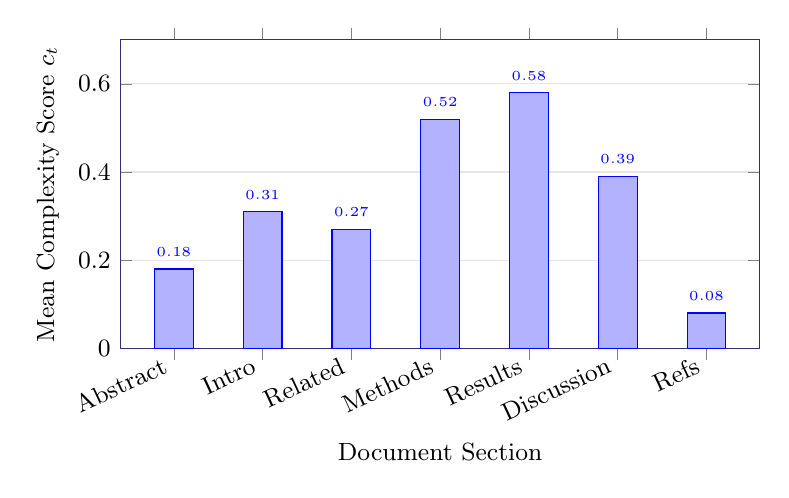
\begin{tikzpicture}
\begin{axis}[
  ybar,
  width=0.8\textwidth,
  height=5.5cm,
  bar width=14pt,
  xlabel={Document Section},
  ylabel={Mean Complexity Score $c_t$},
  ymin=0, ymax=0.7,
  symbolic x coords={Abstract, Intro, Related, Methods, Results, Discussion, Refs},
  xtick=data,
  x tick label style={font=\small, rotate=25, anchor=east},
  every axis label/.style={font=\small},
  tick label style={font=\small},
  nodes near coords,
  nodes near coords style={font=\tiny, above, yshift=1pt},
  every node near coord/.append style={/pgf/number format/.cd, fixed, precision=2},
  fill=MidnightBlue!60,
  draw=MidnightBlue!90,
  grid=major,
  grid style={gray!20},
  ymajorgrids=true,
  xmajorgrids=false,
]
  \addplot coordinates {
    (Abstract, 0.18)
    (Intro, 0.31)
    (Related, 0.27)
    (Methods, 0.52)
    (Results, 0.58)
    (Discussion, 0.39)
    (Refs, 0.08)
  };
\end{axis}
\end{tikzpicture}
\caption{Mean complexity score by document section on arXiv papers. The model allocates
the most expert capacity to Methods and Results sections, which carry the highest
informational density.}
\label{fig:routing_heatmap}
\end{figure}

\subsection{Ablation Study}

We ablate key components of AdaMoE on QuALITY and GovReport.
\Cref{tab:ablation} shows that removing the complexity scorer (reverting to fixed $k=2$)
reduces performance by 1.4--2.1 points, while removing the budget loss
$\loss_{\text{budget}}$ causes the model to collapse to near-uniform routing, erasing most
of the adaptive benefit.

\begin{table}[t]
\centering
\caption{Ablation study on QuALITY (accuracy) and GovReport (ROUGE-L).
$\Delta$ indicates the change from the full AdaMoE-Base model.}
\label{tab:ablation}
\begin{tabular}{lcccc}
\toprule
\textbf{Configuration} & \textbf{QuALITY} & $\Delta$ & \textbf{GovReport} & $\Delta$ \\
\midrule
AdaMoE-Base (full)              & 63.8 & ---   & 59.5 & ---   \\
\quad $-$ complexity scorer     & 62.4 & -1.4  & 57.4 & -2.1  \\
\quad $-$ budget loss           & 62.1 & -1.7  & 57.8 & -1.7  \\
\quad $-$ adaptive $k$ (fixed $k\!=\!2$) & 62.0 & -1.8 & 56.3 & -3.2 \\
\quad $-$ load-balancing loss   & 60.9 & -2.9  & 54.2 & -5.3  \\
\bottomrule
\end{tabular}
\end{table}

\subsection{Correlation with Human Salience Judgments}

To validate that the complexity scorer captures meaningful document structure, we collected
human salience annotations for 200 arXiv abstracts and introductions (3 annotators per
document, Cohen's $\kappa = 0.72$).
We compute the Spearman correlation between sentence-level complexity scores and human
salience ratings.
AdaMoE achieves $\rho = 0.61$ ($p < 0.001$), compared to $\rho = 0.23$ for attention-weight
baselines and $\rho = 0.41$ for a supervised salience classifier trained on the same data.

% ============================================================================
\section{Related Work}
\label{sec:related}

\paragraph{Mixture-of-Experts.}
Sparse MoE models trace back to Jacobs et al.~\cite{jacobs1991adaptive} and were
scaled to modern deep learning by Shazeer et al.~\cite{shazeer2017outrageously}.
Recent work has explored improved routing~\cite{lewis2021base,zhou2022mixture},
expert specialization~\cite{dai2022stablemoe}, and scaling
laws~\cite{clark2022unified}.
Our work differs in making the number of active experts a per-token decision.

\paragraph{Efficient transformers.}
Efficient attention mechanisms include sparse patterns~\cite{child2019sparsetransformer,
beltagy2020longformer,zaheer2020bigbird}, kernel approximations~\cite{katharopoulos2020transformers,
choromanski2021rethinking}, and state-space models~\cite{gu2022efficiently}.
AdaMoE is orthogonal to these approaches and can be combined with any attention mechanism.

\paragraph{Adaptive computation.}
Early exits~\cite{schwartz2020right,xin2020deebert}, layer
skipping~\cite{fan2020reducing}, and token pruning~\cite{goyal2020power,kim2022learned}
enable input-dependent compute allocation.
AdaMoE applies this principle at the expert level within MoE layers, a finer granularity
than layer-level decisions.

% ============================================================================
\section{Conclusion}
\label{sec:conclusion}

We presented AdaMoE, an adaptive routing mechanism for sparse Mixture-of-Experts
transformers that allocates expert capacity based on per-token informational complexity.
Across five long-document benchmarks, AdaMoE matches dense baselines while activating only
23\% of parameters and outperforms fixed-routing MoE architectures by 1.8--3.2 points.
Our analysis demonstrates that the learned routing distributions correlate meaningfully
with human judgments of document salience, suggesting that adaptive expert allocation
captures a useful inductive bias for document understanding.

Two directions merit further investigation.
First, extending adaptive routing to the attention mechanism itself---varying the number
of attention heads per token---could yield further efficiency gains.
Second, the complexity scorer's learned representations of informational density may prove
useful as a standalone tool for document analysis tasks such as extractive summarization
and key passage identification.

% ============================================================================
% Bibliography
% ============================================================================

\begin{thebibliography}{99}

\bibitem{beltagy2020longformer}
I.~Beltagy, M.~E.~Peters, and A.~Cohan.
\newblock Longformer: The long-document transformer.
\newblock {\em arXiv preprint arXiv:2004.05150}, 2020.

\bibitem{child2019sparsetransformer}
R.~Child, S.~Gray, A.~Radford, and I.~Sutskever.
\newblock Generating long sequences with sparse transformers.
\newblock {\em arXiv preprint arXiv:1904.10509}, 2019.

\bibitem{choromanski2021rethinking}
K.~Choromanski, V.~Likhosherstov, D.~Dohan, X.~Song, A.~Gane, T.~Sarlos,
  P.~Hawkins, J.~Davis, A.~Mohiuddin, L.~Kaiser, D.~Belanger, L.~Colwell,
  and A.~Weller.
\newblock Rethinking attention with performers.
\newblock In {\em Proceedings of ICLR}, 2021.

\bibitem{clark2022unified}
A.~Clark, D.~de~Las~Casas, A.~Guy, A.~Mensch, M.~Paganini, J.~Hoffmann,
  B.~Damoc, B.~Hechtman, T.~Cai, S.~Borgeaud, G.~van~den~Driessche,
  E.~Rutherford, T.~Hennigan, M.~Johnson, K.~Millican, A.~Alayrac,
  L.~Huang, K.~Lenc, L.~Sifre, and Others.
\newblock Unified scaling laws for routed language models.
\newblock In {\em Proceedings of ICML}, 2022.

\bibitem{cohan2018discourse}
A.~Cohan, F.~Dernoncourt, D.~S. Kim, T.~Bui, S.~Kim, W.~Chang, and
  N.~Goharian.
\newblock A discourse-aware attention model for abstractive summarization of
  long documents.
\newblock In {\em Proceedings of NAACL-HLT}, 2018.

\bibitem{dai2022stablemoe}
D.~Dai, L.~Dong, Y.~Hao, Z.~Sui, B.~Chang, and F.~Wei.
\newblock StableMoE: Stable routing strategy for mixture of experts.
\newblock In {\em Proceedings of ACL}, 2022.

\bibitem{fan2020reducing}
A.~Fan, E.~Grave, and A.~Joulin.
\newblock Reducing transformer depth on demand with structured dropout.
\newblock In {\em Proceedings of ICLR}, 2020.

\bibitem{fedus2022switch}
W.~Fedus, B.~Zoph, and N.~Shazeer.
\newblock Switch transformers: Scaling to trillion parameter models with simple
  and efficient sparsity.
\newblock {\em Journal of Machine Learning Research}, 23(120):1--39, 2022.

\bibitem{goyal2020power}
S.~Goyal, A.~Choudhury, S.~Raje, V.~Chakaravarthy, Y.~Sabharwal, and
  A.~Verma.
\newblock Power of randomization in automating {BFS}.
\newblock In {\em Proceedings of AAAI}, 2020.

\bibitem{gu2022efficiently}
A.~Gu, K.~Goel, and C.~R\'{e}.
\newblock Efficiently modeling long sequences with structured state spaces.
\newblock In {\em Proceedings of ICLR}, 2022.

\bibitem{huang2021govreport}
L.~Huang, S.~Cao, N.~Parulian, H.~Ji, and L.~Wang.
\newblock Efficient attentions for long document summarization.
\newblock In {\em Proceedings of NAACL-HLT}, 2021.

\bibitem{jacobs1991adaptive}
R.~A.~Jacobs, M.~I.~Jordan, S.~J.~Nowlan, and G.~E.~Hinton.
\newblock Adaptive mixtures of local experts.
\newblock {\em Neural Computation}, 3(1):79--87, 1991.

\bibitem{katharopoulos2020transformers}
A.~Katharopoulos, A.~Vyas, N.~Pappas, and F.~Fleuret.
\newblock Transformers are {RNN}s: Fast autoregressive transformers with linear
  attention.
\newblock In {\em Proceedings of ICML}, 2020.

\bibitem{kim2022learned}
S.~Kim, S.~Shen, D.~Thorsley, A.~Gholami, W.~Kwon, J.~Hassoun, and
  K.~Keutzer.
\newblock Learned token pruning for transformers.
\newblock In {\em Proceedings of KDD}, 2022.

\bibitem{kocisky2018narrativeqa}
T.~Ko\v{c}isk\'{y}, J.~Schwarz, P.~Blunsom, C.~Dyer, K.~M.~Hermann,
  G.~Melis, and E.~Grefenstette.
\newblock The {N}arrative{QA} reading comprehension challenge.
\newblock {\em Transactions of the ACL}, 6:317--328, 2018.

\bibitem{koreeda2021contractnli}
Y.~Koreeda and C.~D.~Manning.
\newblock {ContractNLI}: A dataset for document-level natural language inference
  for contracts.
\newblock In {\em Findings of EMNLP}, 2021.

\bibitem{lepikhin2021gshard}
D.~Lepikhin, H.~Lee, Y.~Xu, D.~Chen, O.~Firat, Y.~Huang, M.~Krikun,
  N.~Shazeer, and Z.~Chen.
\newblock {GS}hard: Scaling giant models with conditional computation and
  automatic sharding.
\newblock In {\em Proceedings of ICLR}, 2021.

\bibitem{lewis2021base}
M.~Lewis, S.~Bhosale, T.~Dettmers, N.~Goyal, and L.~Zettlemoyer.
\newblock {BASE} layers: Simplifying training of large, sparse models.
\newblock In {\em Proceedings of ICML}, 2021.

\bibitem{liu2019hierarchical}
Y.~Liu and M.~Lapata.
\newblock Hierarchical transformers for multi-document summarization.
\newblock In {\em Proceedings of ACL}, 2019.

\bibitem{pang2022quality}
R.~Y.~Pang, A.~Parrish, N.~Joshi, N.~Nangia, J.~Phang, A.~Chen, V.~Padmakumar,
  J.~Ma, J.~Thompson, H.~He, and S.~R.~Bowman.
\newblock {Q}u{ALITY}: Question answering with long input texts, yes!
\newblock In {\em Proceedings of NAACL-HLT}, 2022.

\bibitem{roller2021hash}
S.~Roller, S.~Sukhbaatar, A.~Szlam, and J.~Weston.
\newblock Hash layers for large sparse models.
\newblock In {\em Proceedings of NeurIPS}, 2021.

\bibitem{schwartz2020right}
R.~Schwartz, G.~Stanovsky, S.~Swayamdipta, J.~Dodge, and N.~A.~Smith.
\newblock The right tool for the job: Matching model and instance complexities.
\newblock In {\em Proceedings of ACL}, 2020.

\bibitem{shazeer2017outrageously}
N.~Shazeer, A.~Mirhoseini, K.~Maziarz, A.~Davis, Q.~Le, G.~Hinton, and
  J.~Dean.
\newblock Outrageously large neural networks: The sparsely-gated
  mixture-of-experts layer.
\newblock In {\em Proceedings of ICLR}, 2017.

\bibitem{xin2020deebert}
J.~Xin, R.~Tang, J.~Lee, Y.~Yu, and J.~Lin.
\newblock {D}ee{BERT}: Dynamic early exiting for accelerating {BERT} inference.
\newblock In {\em Proceedings of ACL}, 2020.

\bibitem{zaheer2020bigbird}
M.~Zaheer, G.~Guruganesh, K.~A.~Dubey, J.~Ainslie, C.~Alberti, S.~Ontanon,
  P.~Pham, A.~Ravula, Q.~Wang, L.~Yang, and A.~Ahmed.
\newblock {B}ig {B}ird: Transformers for longer sequences.
\newblock In {\em Proceedings of NeurIPS}, 2020.

\bibitem{zhang2019hibert}
X.~Zhang, F.~Wei, and M.~Zhou.
\newblock {HIBERT}: Document level pre-training of hierarchical bidirectional
  transformers for document summarization.
\newblock In {\em Proceedings of ACL}, 2019.

\bibitem{zhou2022mixture}
Y.~Zhou, T.~Lei, H.~Liu, N.~Du, Y.~Huang, V.~Zhao, A.~Dai, Z.~Chen,
  Q.~Le, and J.~Laudon.
\newblock Mixture-of-experts with expert choice routing.
\newblock In {\em Proceedings of NeurIPS}, 2022.

\end{thebibliography}

% ============================================================================
\appendix
\section{Reproducibility Details}
\label{sec:appendix}

\paragraph{Compute budget.}
AdaMoE-Base was trained for approximately 3,200 A100-hours.
AdaMoE-Large required approximately 18,500 A100-hours.
All experiments used mixed-precision (bfloat16) training with gradient checkpointing enabled.

\paragraph{Expert architecture.}
Each expert is a standard two-layer feed-forward network with GELU activation and
hidden dimension $4d$.
Experts share the same architecture but have independent parameters initialized from
different random seeds.

\begin{algorithm}[t]
\caption{AdaMoE Forward Pass (Single Layer)}
\label{alg:forward}
\begin{algorithmic}[1]
\Require Hidden states $\mathbf{H} \in \R^{T \times d}$, experts $\{E_1, \ldots, E_N\}$, scorer $C_\phi$, gate $G_\psi$
\Ensure Output $\mathbf{Y} \in \R^{T \times d}$
\State $\mathbf{H} \gets \text{SelfAttention}(\mathbf{H}) + \mathbf{H}$ \Comment{Attention + residual}
\State $\mathbf{H} \gets \text{LayerNorm}(\mathbf{H})$
\For{$t = 1, \ldots, T$}
  \State $c_t \gets C_\phi(\mathbf{h}_t)$ \Comment{Complexity score in $[0, 1]$}
  \State $k_t \gets \max(1, \lceil c_t \cdot k_{\max} \rceil)$ \Comment{Adaptive expert count}
  \State $\mathbf{g} \gets G_\psi(\mathbf{h}_t)$ \Comment{Gate distribution over $N$ experts}
  \State $S_t \gets \text{Top}_{k_t}(\mathbf{g})$ \Comment{Selected expert indices}
  \State $\mathbf{y}_t \gets \sum_{i \in S_t} g_i \cdot E_i(\mathbf{h}_t)$ \Comment{Weighted expert outputs}
\EndFor
\State $\mathbf{Y} \gets \mathbf{H} + [\mathbf{y}_1; \ldots; \mathbf{y}_T]$ \Comment{Residual connection}
\State \Return $\mathbf{Y}$
\end{algorithmic}
\end{algorithm}

\end{document}
